\iffalse
	\chapter{2008}
	\author{AI24BTECH11003}
	\section{ph}
\fi

%1
    \item An O$^{16}$ nucleus is spherical and has a charge radius R and a volume $V\equiv\frac{4}{3}\pi R^3$. According to the empirical observations of the charge radii, the volume of the $_{54}Xe^{128}$ nucleus, assumed to be spherical, is
    
    \hfill{(2008)}

        \begin{multicols}{4}
            \begin{enumerate}
                \item $8V$
                \item $2V$
                \item $6.75V$
                \item $1.89V$
            \end{enumerate}
        \end{multicols}

%2
    \item A common emitter transistor amplifier circuit is operated under a fixed bias. In this circuit, the operating point
    
    \hfill{(2008)}
    
            \begin{enumerate}
                \item remains fixed with an increase in temperature.
                \item moves towards cut-off region with an increase in temperature.
                \item moves towards saturation region with a decrease in temperature.
                \item moves towards saturation region with an increase in temperature
            \end{enumerate}

%3
    \item Under normal operating conditions, the gate terminal of an $n$-channel junction field effect transistor (JFET) and an $n$-channel metal oxide semiconductor field effect transistor (MOFSET) are
    
    \hfill{(2008)}

            \begin{enumerate}
                \item both biased with positive potentials
                \item both biased with negative potentials
                \item biased with positive and negative potentials, respectively
                \item biased with negative and positive potentials, respectively
            \end{enumerate}


%4
    \item The eigenvalues of the matrix $\myvec{\cos\theta & -\sin\theta \\ \sin\theta & \cos\theta}$
    
    \hfill{(2008)}
		\begin{multicols}{2}
			\begin{enumerate}
				\item $\frac{1}{2}\brak{\sqrt{3}\pm i}$ when $\theta=45\degree$
				\item $\frac{1}{2}\brak{\sqrt{3}\pm i}$ when $\theta=30\degree$
				\item $\pm1$ since the matrix is unitary
				\item $\frac{1}{\sqrt{2}}\brak{1\pm i}$ when $\theta=30\degree$
			\end{enumerate}
		\end{multicols}

%5
    \item If the Fourier transform $F\left[\delta\brak{x-\alpha}\right]=\exp\brak{-i2\pi\nu a}$, then $F^{-1}\brak{\cos 2\pi a\nu}$ will correspond to 
    
    \hfill{(2008)}

    \begin{multicols}{2}
       \begin{enumerate}
            \item $\delta\brak{x-\alpha}-\delta\brak{x+\alpha}$
            \item a constant
            \item $\frac{1}{2}\left[\delta\brak{x-\alpha}+i\delta\brak{x+\alpha}\right]$
            \item $\frac{1}{2}\left[\delta\brak{x-\alpha}+\delta\brak{x+\alpha}\right]$
        \end{enumerate}
    \end{multicols}
  
%6
    \item If $I=\underset{C}{\oint}dz\ln\brak{z}$, where $C$ is the unit circle taken anticlockwise and $\ln\brak{z}$ is the principal branch of the Logarithmic function, which of the following is correct?
    
    \hfill{(2008)}

    \begin{multicols}{2}
        \begin{enumerate}
            \item $I=0$ by residue theorem
            \item $I$ is not defined since $\ln\brak{z}$ has a branch cut
            \item $I\neq0$
            \item $\underset{C}{\oint}dz\ln\brak{z^2}=2I$
        \end{enumerate}
    \end{multicols}

%7
    \item The value of $\underset{-i}{\overset{i}{\int}}\pi\brak{z+1}dz$ is 
    
    \hfill{(2008)}

        \begin{multicols}{4}
            \begin{enumerate}
                \item $0$
                \item $2\pi i$
                \item $-2\pi i$
                \item $\brak{-1+2i}\pi$
            \end{enumerate}
        \end{multicols}
		
%8
    \item Consider the Bessel equation $\nu=0,\frac{d^2y}{dz^2}+\frac{1}{z}\frac{dy}{dz}+y=0$. Which one of the following statements is correct?
    
    \hfill{(2008)}


            \begin{enumerate}
                \item Equation has regular singular points at $z=0$ and $z=\infty$
                \item Equation has 2 linearly independent solutions that are entire
                \item Equation has an entire solution and a second linearly independent solution singular at $z=0$.
                \item Limit $z\rightarrow\infty$, taken along $x$ axis, exists for both the linearly independent solutions.
            \end{enumerate}


%9
    \item Under a certain rotation of coordinate axes, a rank-1 tensor $\nu_a \brak{a=1,2,3}$ transforms according to the orthogonal transformation defined by the relations $\nu_1'=\frac{1}{\sqrt{2}}\brak{\nu_1+\nu_2};\nu_2'=\frac{1}{\sqrt{2}}\brak{-\nu_1+\nu_2};\nu_3'=\nu_3$. Under the same rotation, a rank-2 tensor $T_{a,b}$ would transform such that
    
    \hfill{(2008)}

        \begin{multicols}{2}
            \begin{enumerate}
                \item $T'_{1,1}=T_{1,1}T_{1,2}$
                \item $T'_{1,3}=T_{1,3}$
                \item $T'_{1,1}=T_{1,1}+2T_{2,2}-T_{2,1}$
                \item $T'_{1,1}=\frac{1}{2}\brak{T_{1,1}+T_{2,2}+T_{1,2}+T_{2,1}}$
            \end{enumerate}
        \end{multicols}

%10
    \item The Lagrangian of a system is given by $L=\frac{1}{2}\dot{q}^2+q\dot{q}-\frac{1}{2}q^2$. It describes the motion of
    
    \hfill{(2008)}

        \begin{multicols}{2}
            \begin{enumerate}
                \item a harmonic oscillator
                \item a damped harmonic oscillator
                \item an anharmonic oscillator
                \item a system with unbounded motion
            \end{enumerate}
        \end{multicols}
        
%11
    \item The moment of inertia tensor of a rigid body is given by $I=\myvec{8&0&-4\\0&4&0\\-4&0&8}$. The magnitude of the moment of inertia about an axis $\hat{n}=\brak{\frac{1}{2},\frac{\sqrt{3}}{2},0}$ is
    
    \hfill{(2008)}

        \begin{multicols}{4}
            \begin{enumerate}
                \item 6
                \item 5
                \item 2
                \item $\frac{8}{3}$
            \end{enumerate}
        \end{multicols}

%12
    \item A hoop of radius R is pivoted at a point on the circumference. The period of small oscillations in the plane of the hoop is 
    
    \hfill{(2008)}

        \begin{multicols}{4}
            \begin{enumerate}
                \item $2\pi\sqrt{\frac{2R}{g}}$
                \item $2\pi\sqrt{\frac{R}{4g}}$
                \item $2\pi\sqrt{\frac{R}{g}}$
                \item $2\pi\sqrt{\frac{9R}{7g}}$
            \end{enumerate}
        \end{multicols}
        
%13
    \item A mass $m$ is constrained to move on a horizontal frictionless surface. It is set in circular motion with radius $r_0$ and angular speed $\omega_0$ by an applied force $\overrightarrow{F}$ communicated through an inextensible thread that passes through a hole on the surface as shown in the figure. This force is suddenly doubled. The magnitude of radial velocity of the mass 
    
    \hfill{(2008)}

    \begin{center}
    \resizebox{0.45\textwidth}{!}{
        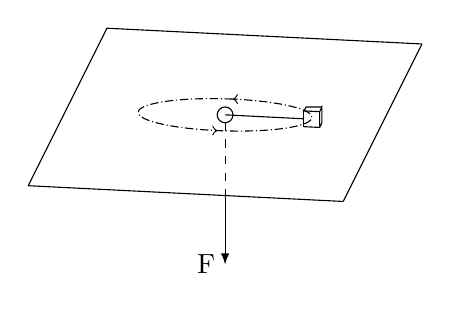
\begin{tikzpicture}
            \draw (0,0) to (4,-0.2);
            \draw (0,0) to (1,2);
            \draw (4,-0.2) to (5,1.8);
            \draw (1,2) to (5,1.8);
            \draw (2.5, 0.9) circle (0.1cm);
            \draw (2.5, 0.9) to (3.5, 0.85);
            \draw (3.5, 0.75) to (3.5, 0.95);
            \draw (3.7, 0.94) to (3.5, 0.95) to (3.53, 1) to (3.73, 1);
            \draw (3.5, 0.75) to (3.7, 0.74) to (3.7, 0.94) to (3.73, 1.00) to (3.73, 0.80) to (3.7, 0.74);
            \draw [black, densely dashdotted] plot [smooth cycle, tension=1] coordinates {(3.6, 0.85) (2.6, 1.1) (1.4, 0.95) (2.4, 0.7)};
            \draw[->] (2.4, 0.7) to ++(0.0004,-0.00002);
            \draw[->] (2.6, 1.1) to ++(-0.0004,+0.00002);
            \draw [black, dashed] (2.5, 0.8) to (2.5, -0.125);
            \draw [black, -latex] (2.5, -0.125) to (2.5, -1) node[left]{F};
        \end{tikzpicture}
    }
\end{center}


            \begin{enumerate}
                \item increases till the mass falls into the hole
                \item decreases till the mass falls into the hole
                \item remains constant
                \item becomes zero at a radius $r_1$ where $0<r_1<r_0$
            \end{enumerate}


%14
    \item For a simple harmonic oscillator the Lagrangian is given by $L=\frac{1}{2}\dot{q}^2-\frac{1}{2}q^2$. If $A\brak{p, q}=\frac{p+iq}{\sqrt{2}}$ and $H\brak{p,q}$ is the Hamiltonian of the system, the Poisson bracket $\left\{ A\brak{p,q},H\brak{p,q}\right\}$ is given by
    
    \hfill{(2008)}

    \begin{multicols}{4}
        \begin{enumerate}
            \item $iA\brak{p,q}$
            \item $A^*\brak{p,q}$
            \item $-iA^*\brak{p,q}$
            \item $-iA\brak{p,q}$
        \end{enumerate}
    \end{multicols}

%15
    \item A plane electromagnetic wave is given by $E_0\brak{\hat{x}+e^{i\delta} \hat{y}}\exp\left\{i\brak{kz-\omega t}\right\}$. At a given location, the number of times $\hat{E}$ vanishes in one second is
    
    \hfill{(2008)}


            \begin{enumerate}
                \item An integer near $\frac{\omega}{\pi}$ when $\delta=n\pi$ and zero when $\delta\neq n\pi$, $n$ is integer
                \item An integer near $\frac{\omega}{\pi}$ and is independent of $\delta$
                \item An integer near $\frac{\omega}{2\pi}$ when $\delta=n\pi$ and zero when $\delta\neq n\pi$, $n$ is integer
                \item An integer near $\frac{\omega}{2\pi}$ and is independent of $\delta$
            \end{enumerate}


%16
    \item A dielectric sphere is placed in a uniform electrical field directed along the positive $y$-axis. Which of the following represents correct equipotential surfaces?
    
    \hfill{(2008)}

        \begin{multicols}{2}
            \begin{enumerate}
                \item 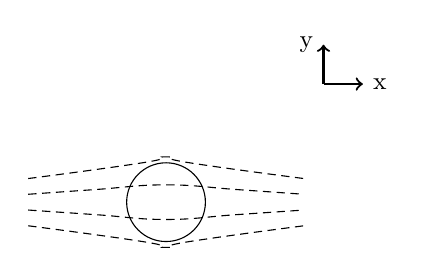
\begin{tikzpicture}
    \draw [black, densely dashed] plot [smooth, tension=0.75] coordinates {(0.25,-0.1) (1.125,-0.16) (2,-0.22) (2.875,-0.16) (3.75,-0.1)};
    \draw [black, densely dashed] plot [smooth, tension=0.75] coordinates {(0.25,0.1) (1.1,0.16) (2,0.22) (2.9,0.16) (3.75,0.1)};
    \draw [black, densely dashed] plot [smooth, tension=1] coordinates {(0.25,0.3) (1.7,0.5) (2,0.575) (2.3,0.5) (3.75,0.3)};
    \draw [black, densely dashed] plot [smooth, tension=1] coordinates {(0.25,-0.3) (1.7,-0.5) (2,-0.575) (2.3,-0.5) (3.75,-0.3)};
    \draw (2,0) circle (0.5cm);

    \draw [black, thick, ->] (4, 1.5) to (4, 2) node[left]{\small y};
    \draw [black, thick, ->] (4, 1.5) to (4.5, 1.5) node[right]{\small x};
\end{tikzpicture}
                \item 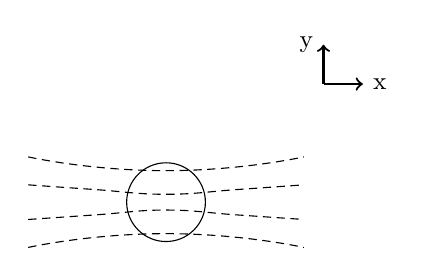
\begin{tikzpicture}
    \draw [black, densely dashed] plot [smooth, tension=0.75] coordinates {(0.25,-0.22) (1.125,-0.16) (2,-0.1) (2.875,-0.16) (3.75,-0.22)};
    \draw [black, densely dashed] plot [smooth, tension=0.75] coordinates {(0.25,0.22) (1.1,0.16) (2,0.1) (2.9,0.16) (3.75,0.22)};
    \draw [black, densely dashed] plot [smooth, tension=1] coordinates {(0.25,0.575) (2,0.4) (3.75,0.575)};
    \draw [black, densely dashed] plot [smooth, tension=1] coordinates {(0.25,-0.575) (2,-0.4) (3.75,-0.575)};
    \draw (2,0) circle (0.5cm);

    \draw [black, thick, ->] (4, 1.5) to (4, 2) node[left]{\small y};
    \draw [black, thick, ->] (4, 1.5) to (4.5, 1.5) node[right]{\small x};
\end{tikzpicture}
                \item 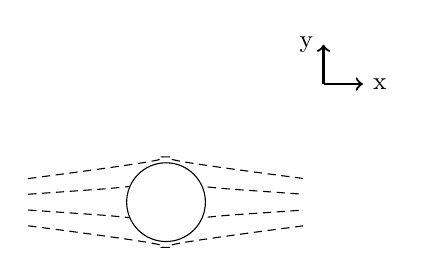
\begin{tikzpicture}
    \draw [black, densely dashed] plot [smooth, tension=0.75] coordinates {(0.25,-0.1) (1.125,-0.16) (2,-0.22) (2.875,-0.16) (3.75,-0.1)};
    \draw [black, densely dashed] plot [smooth, tension=0.75] coordinates {(0.25,0.1) (1.1,0.16) (2,0.22) (2.9,0.16) (3.75,0.1)};
    \draw [black, densely dashed] plot [smooth, tension=1] coordinates {(0.25,0.3) (1.7,0.5) (2,0.575) (2.3,0.5) (3.75,0.3)};
    \draw [black, densely dashed] plot [smooth, tension=1] coordinates {(0.25,-0.3) (1.7,-0.5) (2,-0.575) (2.3,-0.5) (3.75,-0.3)};
    \filldraw[fill=white, draw=black] (2,0) circle (0.5cm);

    \draw [black, thick, ->] (4, 1.5) to (4, 2) node[left]{\small y};
    \draw [black, thick, ->] (4, 1.5) to (4.5, 1.5) node[right]{\small x};
\end{tikzpicture}
                \item \resizebox{0.8\columnwidth}{!}{%
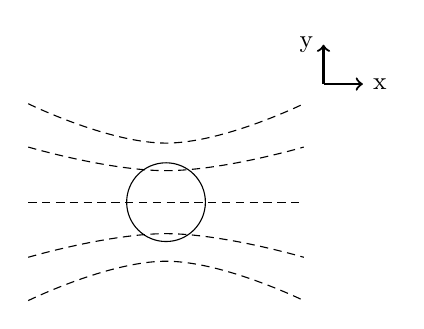
\begin{tikzpicture}
    \draw [black, densely dashed] plot [smooth, tension=0.75] coordinates {(0.25,-0.7) (2,-0.4) (3.75,-0.7)};
    \draw [black, densely dashed] plot [smooth, tension=0.75] coordinates {(0.25,0.7) (2,0.4) (3.75,0.7)};
    \draw [black, densely dashed] plot [smooth, tension=1] coordinates {(0.25,0) (2,0) (3.75,0)};
    \draw [black, densely dashed] plot [smooth, tension=0.75] coordinates {(0.25,1.25) (2,0.75) (3.75,1.25)};
    \draw [black, densely dashed] plot [smooth, tension=0.75] coordinates {(0.25,-1.25) (2,-0.75) (3.75,-1.25)};
    \draw (2,0) circle (0.5cm);

    \draw [black, thick, ->] (4, 1.5) to (4, 2) node[left]{\small y};
    \draw [black, thick, ->] (4, 1.5) to (4.5, 1.5) node[right]{\small x};
\end{tikzpicture}
}
            \end{enumerate}
        \end{multicols}

%17
    \item A rod of length $L$ with uniform charge density $\lambda$ per unit length is in the $xy$-plane and rotating about $z$-axis passing through one of its edge with an angular velocity $\overrightarrow{\omega}$ as shown in the figure below. $\brak{\hat{r}, \hat{\phi}, \hat{z}}$ refer to the unit vectors at $Q$, $\overrightarrow{A}$ is the vector potential at a distance $d$ from the origin $O$ along $z$-axis for $d>>L$ and $\overrightarrow{J}$ is the current density due to the motion of the rod. Which of the following statements is correct?
    
    \hfill{(2008)}

    \begin{center}
        
\resizebox{0.35\textwidth}{!}{
\begin{tikzpicture}
    \centering
    \draw [black, -latex] (0,0) node[anchor = south west]{O} to (0,5) node[above]{z};
    \draw [black, -latex] (0,0) to (4,0) node[right]{y};
    \draw [black, -latex] (0,0) to (-2,-2) node[below]{x};
    \draw [black, -latex] (0,0) to (2.2,-2.2) node[right]{$\hat{r}$};
    \draw [black, very thick] (0,0) to (1.54, -1.54) node[right]{\small Q};
    \draw [black, dashed, <-] (-0.2,0) to (-0.2, 1.6) node[above]{$d$};
    \draw [black, dashed, ->] (-0.2, 2.1) to (-0.2, 3.8);
    \draw [black, dashed, <->] (-0.1, -0.2) to node[below]{\small $L$} (1.44, -1.74);
    \draw [black, -latex] plot [smooth, tension=1] coordinates {(0.15, 4.6) (0, 4.65) (-0.15, 4.55) (0, 4.45) (0.1, 4.5)} node[right]{\small $\omega$};
    \draw [black, -latex] plot [smooth, tension=1] coordinates {(-0.25, -0.25) (0, -0.3) (0.275, -0.275)};
    \filldraw[black] (0,3.8) circle (2pt) node[right]{$P$};
    \node [font=\small] at (-0.2, -0.45) {$\phi$};
\end{tikzpicture}
}

    \end{center}

    \begin{multicols}{2}
        \begin{enumerate}
            \item $\overrightarrow{J}$ along $\hat{r}$; $\overrightarrow{A}$ along $\hat{z}$; $\abs{\overrightarrow{A}}\propto\frac{1}{d}$
            \item $\overrightarrow{J}$ along $\hat{\phi}$; $\overrightarrow{A}$ along $\hat{\phi}$; $\abs{\overrightarrow{A}}\propto\frac{1}{d^2}$
            \item $\overrightarrow{J}$ along $\hat{r}$; $\overrightarrow{A}$ along $\hat{z}$; $\abs{\overrightarrow{A}}\propto\frac{1}{d^2}$
            \item $\overrightarrow{J}$ along $\hat{\phi}$; $\overrightarrow{A}$ along $\hat{\phi}$; $\abs{\overrightarrow{A}}\propto\frac{1}{d}$
        \end{enumerate}
    \end{multicols}

